\subsection{Scalability and Benchmarking results}
%\red{Yangkang}

During a large-scale inversion, the proportion of computational time spend to
simulate wave propagation mandates the solver to be performant and to scale
well.
Figure~\ref{fig:s480} shows \texttt{SPECFEM3D\_GLOBE} strong scaling results
for simulations running on multiple GPUs with a shortest period of 9\,s. It
demonstrates that very close to ideal efficiency can be achieved with a minimum
size of about 100\,MB of data per GPU. Thus, the code exhibits excellent scalability
and can be run with almost ideal code performance in part because communications
are almost entirely overlapped with calculations. Also note that the average
elapsed calculation time per time-step is inversely proportional to the number
of GPUs whether one uses a single MPI process per GPU or two MPI processes. This
indicates that we can run multiple MPI processes on a single GPU without loss of
performance. Depending on the number of simultaneous seismic events that we want
to simulate and the expected maximum time-to-solution, these benchmarks help us
select both the optimal number of GPUs and the organization of the MPI tasks
across them. Scalability improves as the scale of the simulation becomes larger
and larger. Though scalability performance at the lowest resolution (27~s) is
not optimal (Figures~\ref{fig:s160unq} and~\ref{fig:s160nounq}), as the
resolution increases to 9~s scalability performance is very close to
ideal (Figures~\ref{fig:s480} and~\ref{fig:s480nounq}). It should also be
admitted that as the number of MPI tasks used in the simulation increases
---though scalability performance is not affected--- the overall performance of
each GPU node will be slightly decreased. This is because communications
between MPI processes on each node will slightly slow down the computation.

\begin{figure}
  \centering
  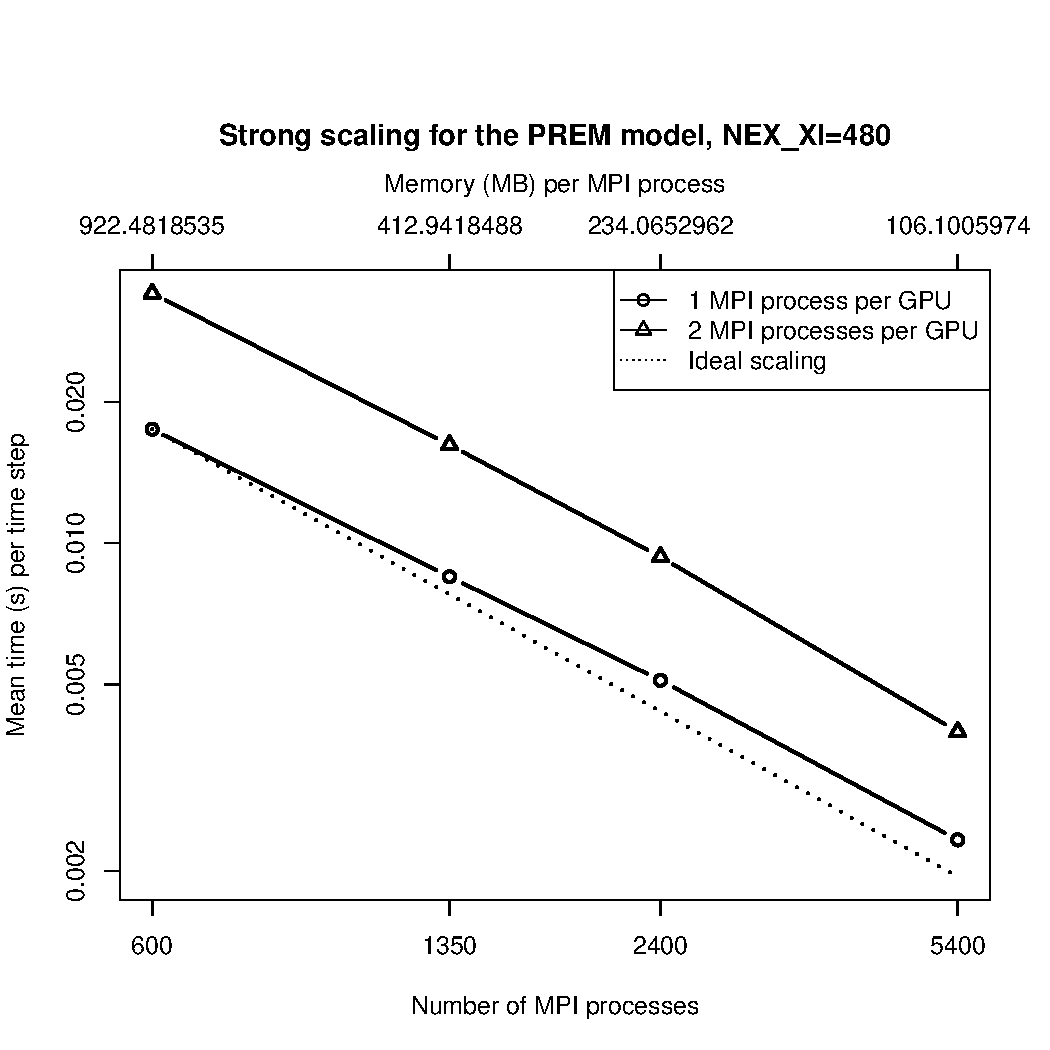
\includegraphics[width=0.8\textwidth]{ch-workflow/figures/s480}
  \caption[Strong scaling of SPECFEM3D GLOBE for the PREM Earth model on Titan for 9\,s minimum period]
  {Strong scaling for the spherically symmetric PREM Earth model on Titan for a minimum seismic
	period of 9\,s. The mesh is comprised of \~\,25 million elements for this
	resolution. Values are plotted against the number of MPI processes. }
   \label{fig:s480}
\end{figure}

Figure \ref{fig:weak} shows \texttt{SPECFEM3D\_GLOBE} weak scaling test results
for an increasing problem size while keeping the
work load for each MPI process almost the same. Weak scaling tests are a bit
unusual for \texttt{SPECFEM3D\_GLOBE}. What we do is find a
setup where slices will have more or less the same number of elements, then
correct the timing by dividing the actual number of elements per slice and
multiply with the setup which we take as a reference. It can be observed from
the weak scaling plot that parallel efficiency for GPU simulations is excellent
and scales within 95\% of the ideal runtimes across all benchmark sizes.
Comparing weak scaling performances between GPU and CPU-only simulations on a
Titan node, i.e., a K20x GPU (Kepler) versus 16 CPU-cores (AMD Interlagos), we
see a speedup factor of the GPU simulations of $\sim$18x for the chosen mesh
sizes. For high-end Intel Xeons microprocessor or IBM Power microprocessor, the
speedup factor of the GPU simulation may not be as high as 18x. To make
\texttt{SPECFEM3D\_GLOBE} ready for next-generation supercomputers, e.g.,
GPU-based machines with high-end microprocessors, continuous work should be
carried out in order to maintain a high speedup factor for GPU simulations. Our
scaling results indicate that asynchronous message passing is nearly perfect in
hiding network latency on Titan. Note that this becomes more of a challenge for
smaller mesh sizes, where the percentage of outer elements increases compared to
inner elements, but such small meshes are never used in practice.
\begin{figure}
  \centering
  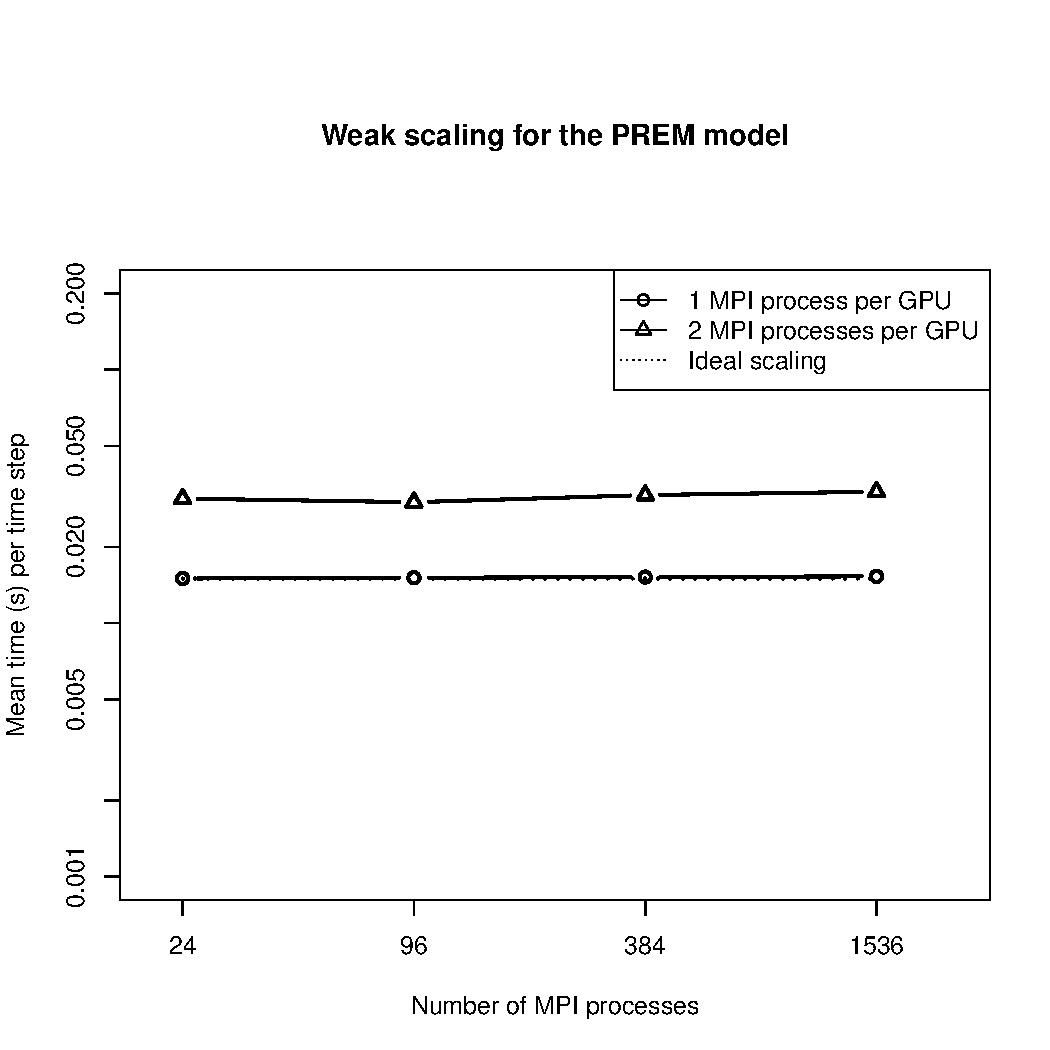
\includegraphics[width=0.8\textwidth]{ch-workflow/figures/weak}
  \caption[Weak scaling of SPECFEM3D GLOBE for the PREM Earth model on Titan for 9\,s minimum period]
  {Weak scaling for the PREM Earth model on Titan. Performance is measured
	as the averaged mean time for each time step. The same work load is applied to
	each MPI process in different cases.}
   \label{fig:weak}
\end{figure}

%\subsubsection{Performance}
%\red{Yangkang}

%\texttt{SPECFEM3D\_GLOBE} parallelization extensively relies on the analytical decomposition of a cubed-sphere mesh, splitting the mesh into partitions with close-to-perfect load balancing and assigning a single partition to a single MPI process. This coarse domain decomposition parallelism may even include a finer level of parallelism inside each domain. For CPU-only computations we carefully and thoroughly optimized the main calculations routines to allow compilers to fully vectorize most of the critical loops. To address accelerators such as GPUs, and eventually Intel Xeon Phi, we rely on BOAST, and open-source source-to-source compiler to generate either CUDA or OPENCL from kernels defined in Ruby. Our experience shows that this gives the same level of performance as programming the SPECFEM3D computation kernels directly in CUDA, but with much improved portability. To date \texttt{SPECFEM3D\_GLOBE} supports OpenMP only for a few routines. OpenMP support was partially added mostly to assess software performance of the code on Xeon Phi accelerators.

%\subsection{Benchmarking results}
%\red{Yangkang}
%Scaling plots, w/ w/o undo attenuation, with varying number of stations.

Next,
we discuss scaling results for low- and high-resolution simulations.
We anticipate that the scalability of low-resolution
simulations will be worse, since the
computing resources of each node will not be
effectively used and MPI communication costs will take up a larger percentage of
the total computation time.
An additional issue is that accurate calculation of the gradient of the misfit function requires full attenuation.
This involves storage of snapshots of the forward wavefield which are read back during the
adjoint simulation, leading to increased I/O.
We expect this additional I/O to adversely affect performance.

Figures~\ref{fig:s160unq} and~\ref{fig:s160nounq} show strong scaling tests
for a low-resolution model (minimum period of 27\,s) with
and without full attenuation, respectively. In each figure, the two
diagrams show the scaling results for 1 and 2 MPI tasks per GPU node. The
scalability does not change as the number of MPI tasks increases. However, when
the number of GPU tasks increases from 1 to 2, the processing time per time step
doubles. The scalability does not change wether or not we are considering full attenuation.  As
anticipated, when considering full attenuation the processing time per time step is a
bit longer than when not considering full attenuation. Table~\ref{tbl:comp160} shows a
comparison of processing time per time step in two different cases for a different
number of MPI processes. Processing time with full attenuation is a bit longer than without.

Figures~\ref{fig:s256unq} and~\ref{fig:s256nounq} show strong scaling tests
for a medium resolution model (minimum period of 17\,s)
in two different situations: with and without full attenuation. The
scalability in the two cases is similar, except that
when considering full attenuation the scalability is a bit better than that of the
opposite case. The number of MPI processes still does not affect scalability
 but is inversely proportional to computational performance.
Compared to the 27~s case, the
17~s simulation shows scalability. Processing efficiency with
full attenuation is also a bit lower than that of without full attenuation, as
shown in table \ref{tbl:comp256}.

Figure~\ref{fig:s480} shows strong scaling tests for 9~s resolution with
full attenuation. Figure~\ref{fig:s480nounq} is the same test without
full attenuation. It is obvious that scalability is close to ideal in
both cases. Comparing the actual processing time for the two cases, as shown in
Table~\ref{tbl:comp480}, we conclude again that full attenuation
causes slightly lower efficiency.

\begin{table}[]
\centering
  \caption[Processing time with and without full attenuation at 27~s resolution]
  {\small{Comparison of processing time per time step with and without full 
    attenuation (27~s resolution).}}
\label{tbl:comp160}
    \begin{tabular}{lccccc}
	  \tch{No.\ of MPI processes} & 24 & 96 & 150 & 600   &  2400			       		 \\
    \midrule
	  \tch{With full attenuation} & 0.025 & 0.00679 & 0.00462 & 0.00174 &0.00148 \\
    \tch{Without full attenuation} & 0.025 & 0.00678 &0.00462 &0.00171 & 0.00135		       		 \\
    \end{tabular}
 \end{table}

\begin{table}[]
\centering
  \caption[Processing time with and without full attenutation at 17~s resolution]
    {\small{Comparison of processing time per time step with and without
      full attenuation (17~s resolution).}}
\label{tbl:comp256}
    \begin{tabular}{lccccc}
	  \tch{No.\ of MPI processes} & 96 & 384 & 1536 & 6144 		       		 \\
    \midrule
	  \tch{With full attenuation} & 0.0194 &0.00542 & 0.0226 & 0.0189 \\
    \tch{Without full attenuation} & 0.0193 & 0.00490 & 0.0023 & 0.00171		       		 \\
    \end{tabular}
 \end{table}

 \begin{table}[]
\centering
   \caption[Processing time with and without full attenuation at 9~s resolution]
   {\small{Comparison of processing time per time step with and without
      full attenuation (9~s resolution).}}
\label{tbl:comp480}
     \begin{tabular}{lcccc}
	  \tch{No.\ of MPI processes} & 600 & 1350 & 2400 & 5400 		       		 \\
    \midrule
	  \tch{With full attenuation} & 0.0175 &0.00848 & 0.0051 & 0.00233 \\
    \tch{Without full attenuation} & 0.017 & 0.00827 & 0.005 & 0.00229	       		 \\
    \end{tabular}
 \end{table}

\begin{figure}
  \centering
  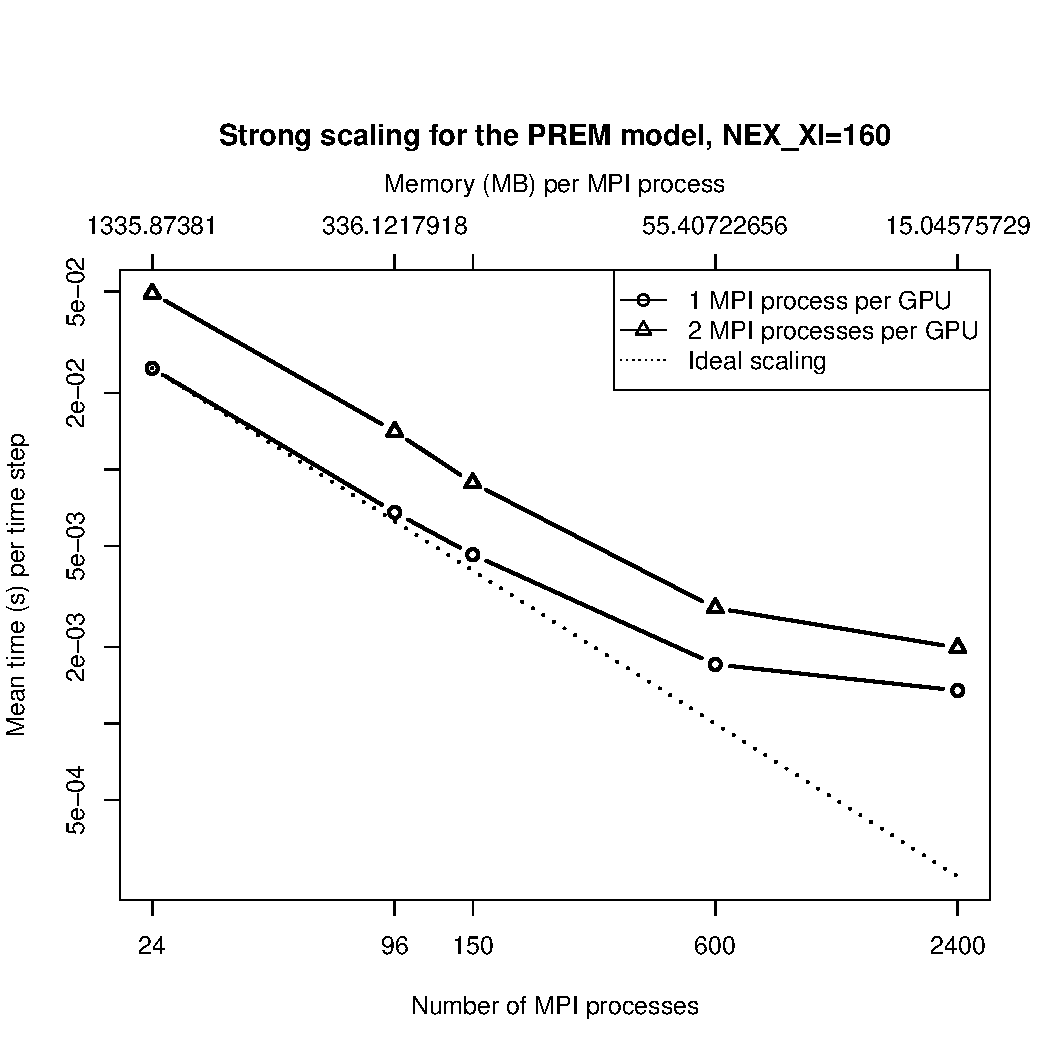
\includegraphics[width=0.8\textwidth]{ch-workflow/figures/s160unq}
  \caption[Strong scaling of SPECFEM3D GLOBE for the PREM Earth model on Titan for 27\,s minimum period with full attenuation]
	{Strong scaling for the PREM Earth model on Titan for a minimum seismic
	period of 27\,s with full attenuation. Values are plotted
	against the number of MPI processes. }
   \label{fig:s160unq}
\end{figure}


\begin{figure}
  \centering
  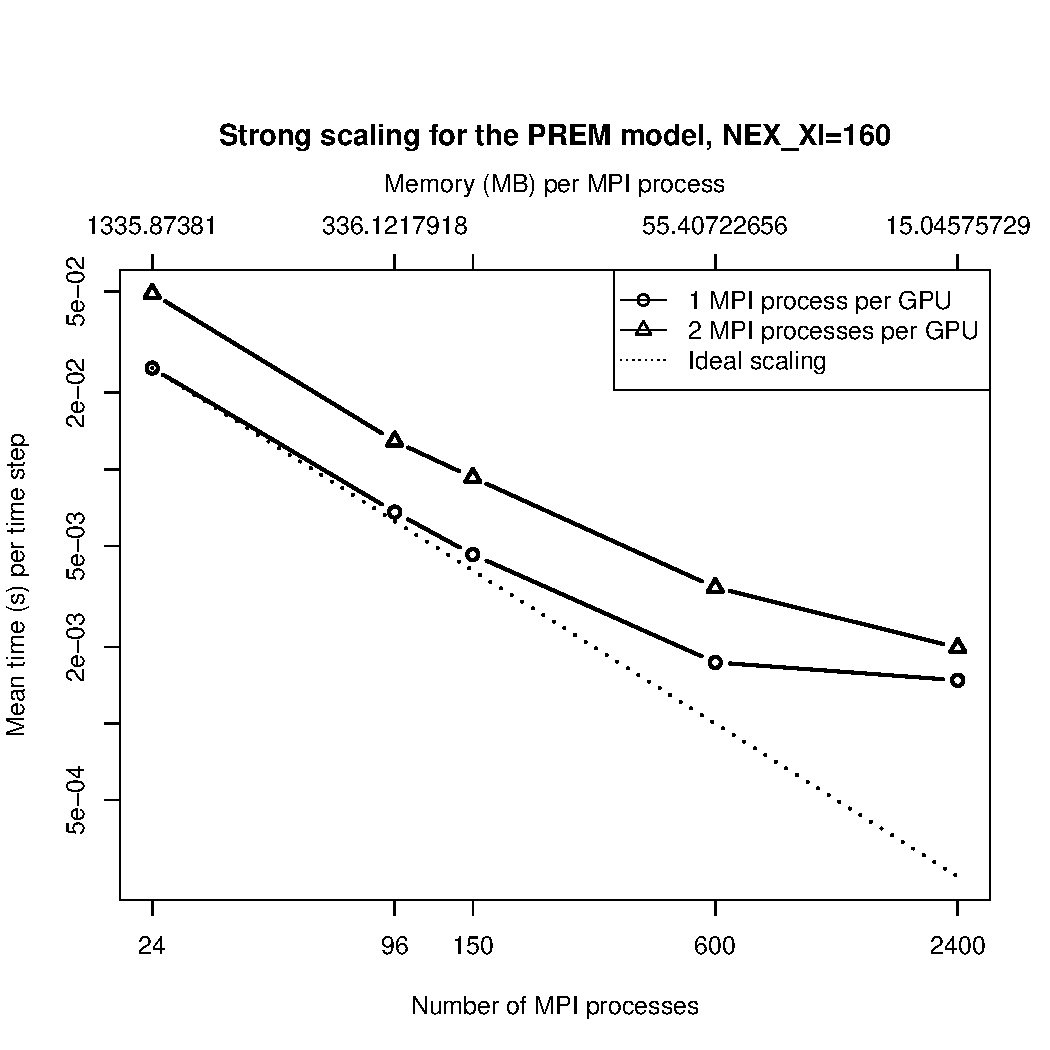
\includegraphics[width=0.8\textwidth]{ch-workflow/figures/s160nounq}
  \caption[Strong scaling of SPECFEM3D GLOBE for the PREM Earth model on Titan for 27\,s minimum period w/o ffull attenuation]
	{Strong scaling for the PREM model on Titan for a minimum seismic
	period of 27\,s in the case of without \emph{full attenuation}.
  Values are plotted against the number of MPI processes. }
   \label{fig:s160nounq}
\end{figure}


\begin{figure}
  \centering
  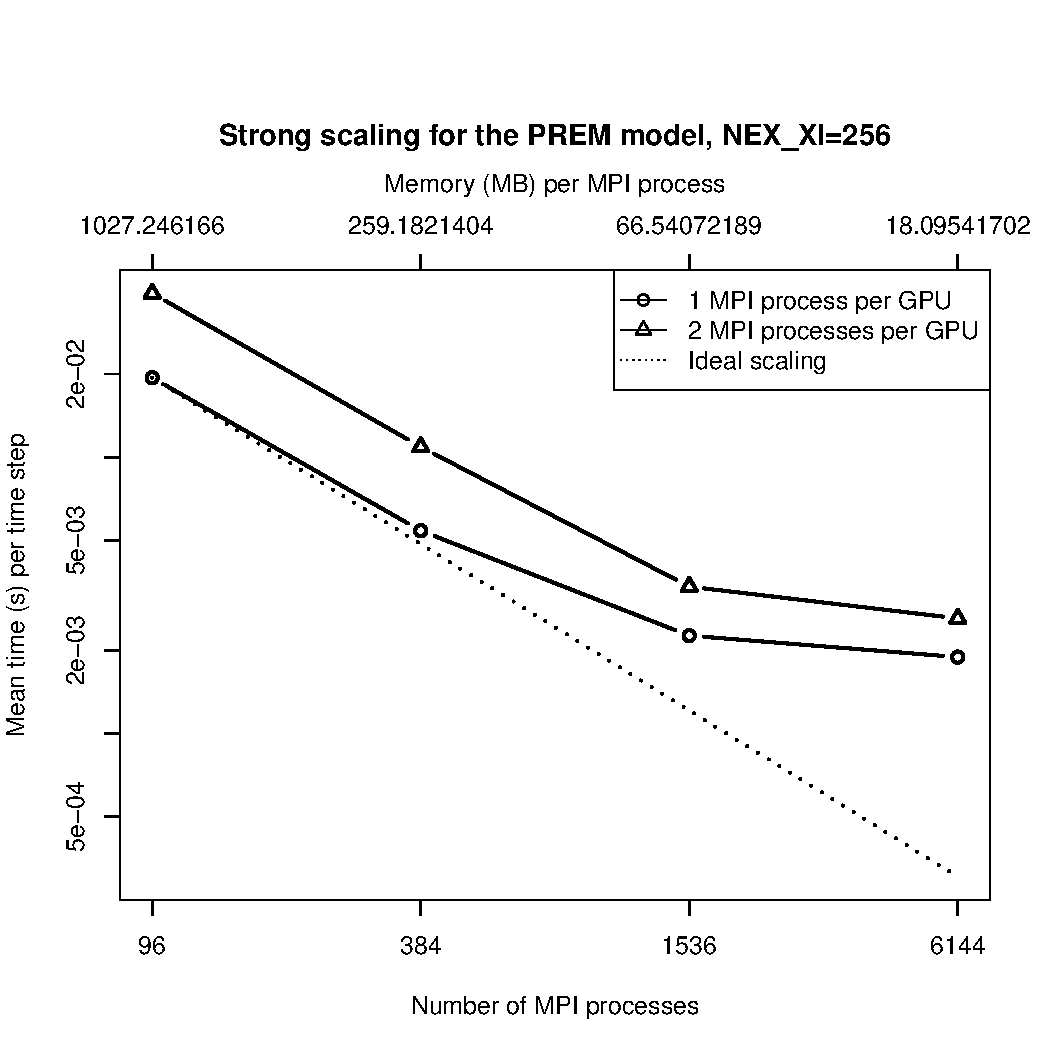
\includegraphics[width=0.8\textwidth]{ch-workflow/figures/s256unq}
  \caption[Strong scaling of SPECFEM3D GLOBE for the PREM Earth model on Titan for 17\,s minimum period with
  full attenuation]
	{Strong scaling for the PREM model on Titan for a minimum seismic
	period of 17\,s in the case of with \emph{full attenuation}. Values are plotted
	against the number of MPI processes. }
   \label{fig:s256unq}
\end{figure}


\begin{figure}
  \centering
  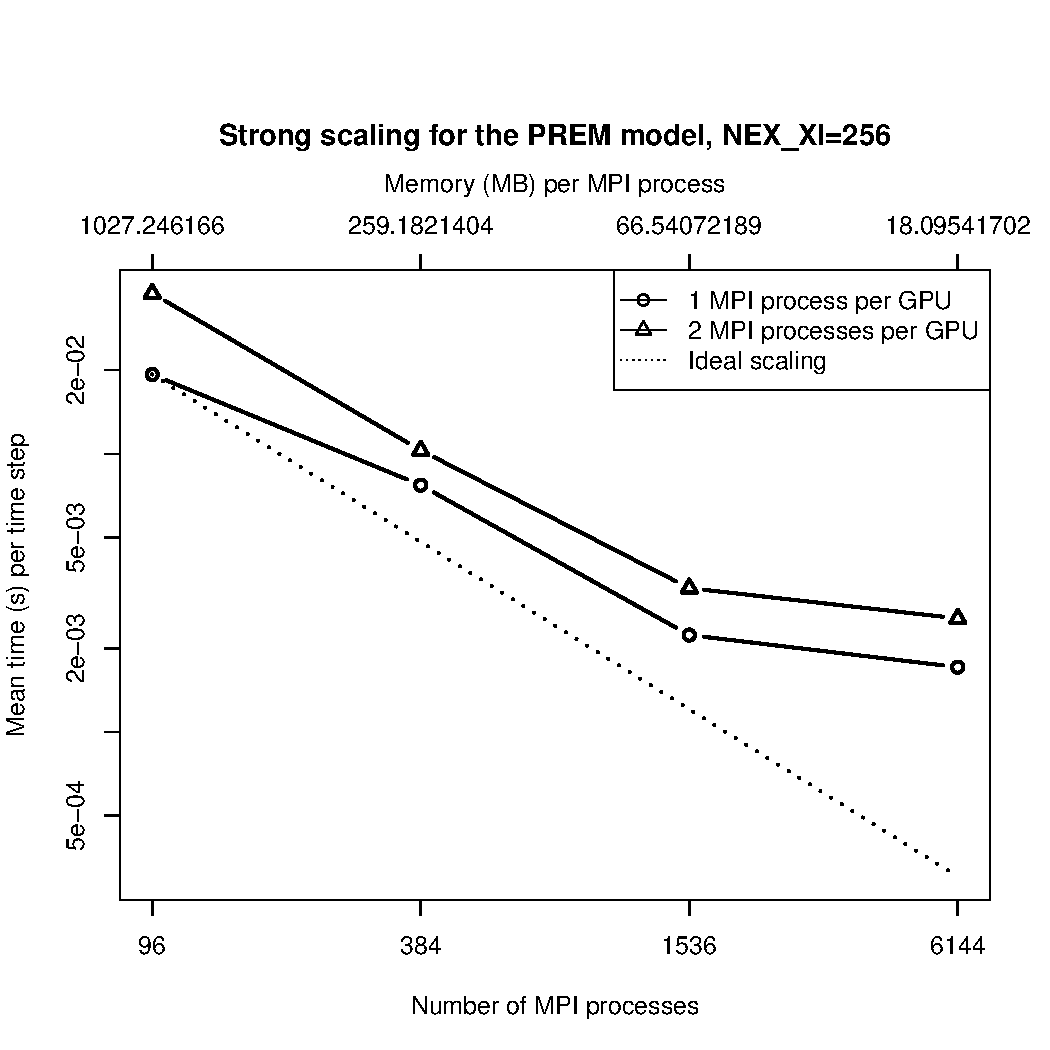
\includegraphics[width=0.8\textwidth]{ch-workflow/figures/s256nounq}
  \caption[Strong scaling of SPECFEM3D GLOBE for the PREM Earth model on Titan for 17\,s minimum period w/o
  full attenuation]
	{Strong scaling for the PREM model on Titan for a minimum seismic
	period of 17\,s in the case of without \emph{full attenuation}.
  Values are plotted against the number of MPI processes. }
   \label{fig:s256nounq}
\end{figure}

\begin{figure}
  \centering
  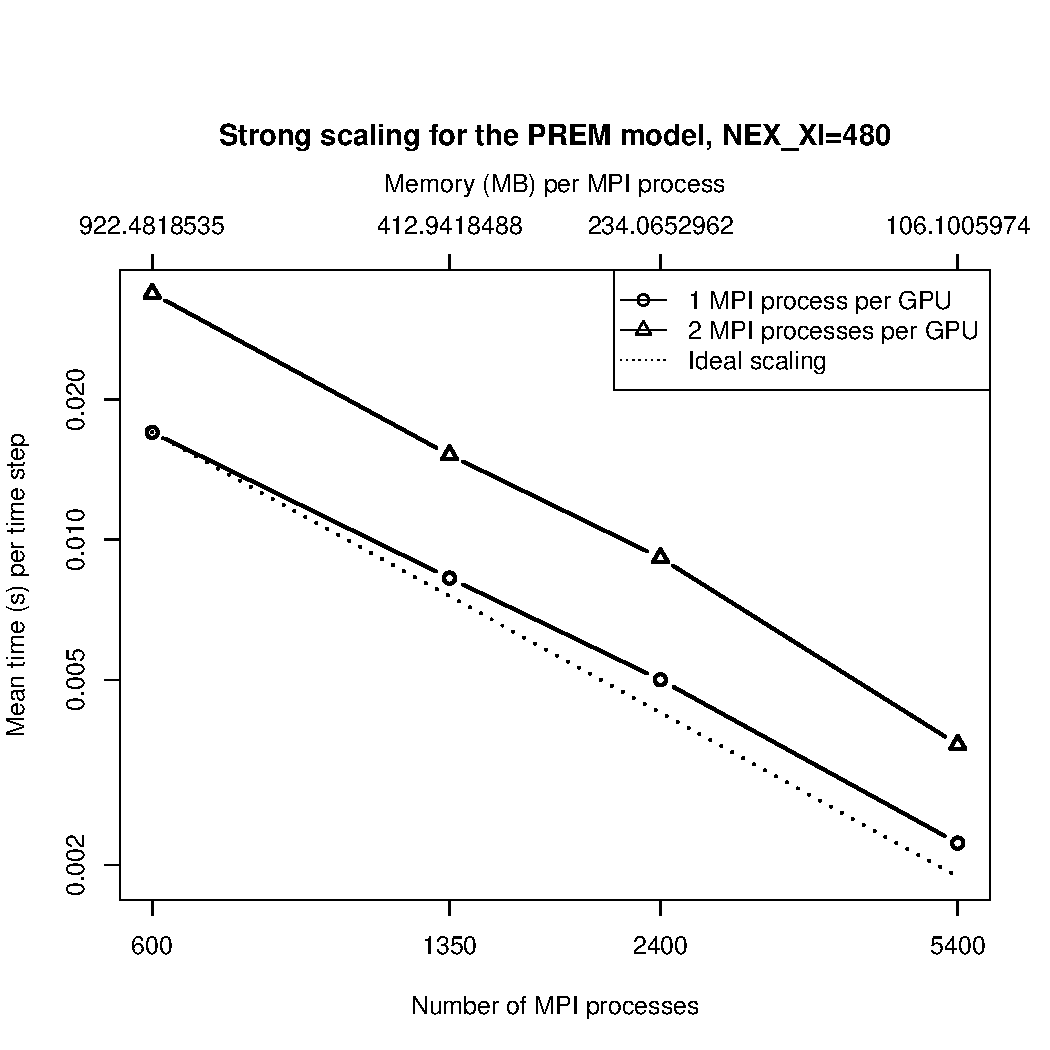
\includegraphics[width=0.8\textwidth]{ch-workflow/figures/s480nounq}
  \caption[Strong scaling of SPECFEM3D GLOBE for the PREM Earth model on Titan for 9\,s minimum period w/o
  full attenuation]
	{Strong scaling for the PREM model on Titan for a minimum seismic
   period of 9\,s in the case of without \emph{full attenuation}.
   Values are plotted against the number of MPI processes. }
   \label{fig:s480nounq}
\end{figure}

We compare the processing time per time step for different output data formats,
including ASDF, our newly design modern seismic data file format (see
Section~\ref{sec:asdf}). Whether or not we use ASDF, the
processing time per time step is almost unaffected.
This observation is encouraging, because when we enjoy the benefits of
ASDF we do not lose the superb scalability performance of the code.
We
also compare scalability performance with respect to the number of receivers.
We find that the number of receivers does not influence scalability of 
\texttt{SPECFEM3D\_GLOBE}. This indicates that as the global
seismographic network becomes denser and denser, scalability will not degrade.

In order to prepare \texttt{SPECFEM3D\_GLOBE} for the next generation
supercomputers, e.g., `Summit', code improvements should be done to ensure a
linear speed up of GPU simulations to at least 20\,\% of current Titan nodes
($\sim$3,600 MPI processes) for both high-resolution and medium-resolution
simulations. High-resolution simulations ($\sim$9\,s) have already demonstrated
perfect scalability to at least 5,400 nodes, which ensures a stable
application for the intermediate future. 
